\newpage
\section{2019秋}

\setcounter{yearcounter}{2019}
% \setcounter{page}{1}


\subsection{微分積分}
\prob{
  $y=x^2e^{-x}$のすべての臨界点(停留点)を求め、極値が最大値か最小値かを判定せよ。
}
\begin{ans*}
  ${}$
  \begin{gather}
    \frac{dy}{dx}
    = x(2 - x)e^{-x}
  \end{gather}
  および
  \begin{gather}
    \lim_{x\to-\infty} y(x) = \infty,\,\lim_{x\to\infty}y(x) = 0
  \end{gather}
  より増減表は下図
  \begin{table}[H]
  \centering
  \begin{tabular}{c||cccccc}
  \toprule
    $x$ & $\cdots$ & 0 & $\cdots$ & 2 & $\cdots$ & ($\infty$)  \\
  \midrule
    \dm{\frac{dy}{dx}} & $-$ & 0 & $+$ & 0 & $-$ & ($\to 0$) \\
  \midrule
    $y$ & $\searrow$ & 0 & $\nearrow$ & $\frac{4}{e^2}$ & $\searrow$ & ($\to 0$) \\
  \bottomrule
  \end{tabular}\end{table}
  % pic
  ゆえに極小値$y(0)$は最小値で、極大値$y(2)$は最大値ではない。
\end{ans*}

\prob{
  次の級数が収束するか発散するかを調べよ。
  \begin{gather}
    \frac{1}{2} + \frac{1}{2} + \frac{3}{8} + \frac{1}{4} + \cdots
  \end{gather}
}
この与えられ方は一意に定まらないと思われます。
ので、一般項を類推することで解答とします。

\begin{ans*}
  ${}$
  与えられた級数が
  \begin{gather}
    \sum_{n=1}^{\infty}\frac{n}{2^n}
  \end{gather}
  と等価であると推測する。
  ここに\dm{a_{n} = \frac{n}{2^n}}とおくと、
  \begin{gather}
    \left| \frac{a_{n+1}}{a_{n}} \right| = \left| \frac{n+1}{2n} \right| \lra \frac{1}{2} \quad(n\to\infty)
  \end{gather}
  より、この級数は収束する。
\end{ans*}

\prob{
  次の線積分を求めよ。
  \begin{gather}
    L = \oint_{C} (2xy\,dy - x^2\,dx)
  \end{gather}
  ここで、$C$は、図に示すように頂点が
  $\rm{O}(0,0),\,\rm{A}(1,0),\,\rm{B}(1,1)$の三角形の3辺で構成される。

  \begin{figure}[H]\centering
    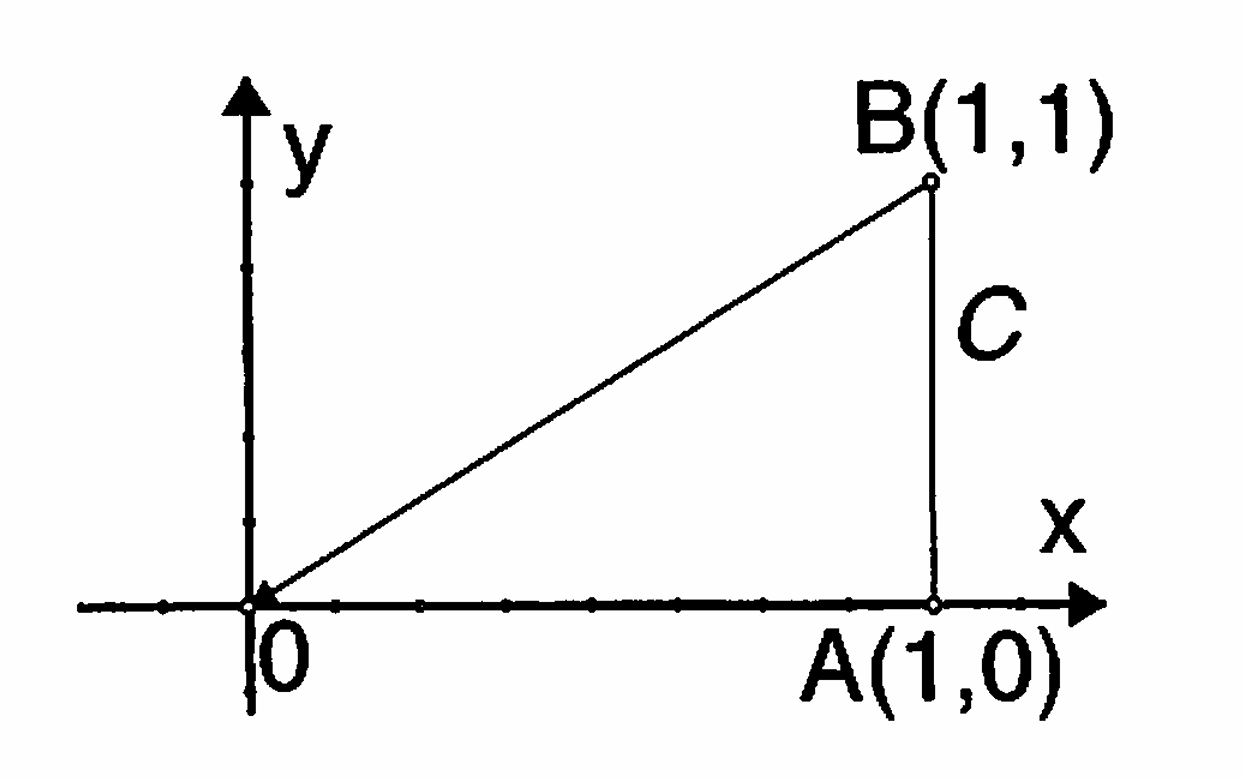
\includegraphics[width=.35\linewidth]{./src/fig/Basic/B_2019_autumn_1-3.png}
  \end{figure}
}

\begin{ans*}
  ${}$
  線分$\rm{OA},\,\rm{AB},\,\rm{BO}$はパラメーター$t_{1},\,t_{2},\,t_{3}$を用いて表すと
  \begin{align}
    \rm{OA}&\colon
    \begin{dcases*}
      x = t_{1} \\
      y = 0
    \end{dcases*} \quad 0\leq t_{1} \leq 1 \\
    \rm{AB}&\colon
    \begin{dcases*}
      x = 1 \\
      y = t_{2}
    \end{dcases*} \quad 0\leq t_{2} \leq 1 \\
    \rm{BO}&\colon
    \begin{dcases*}
      x = 1 - t_{3} \\
      y = 1 - t_{3}
    \end{dcases*} \quad 0\leq t_{3} \leq 1
  \end{align}
  と表せる。
  ここに、与えられた周回積分は
  \begin{gather}
    \oint_{C} = \int_{\rm{OA}} + \int_{\rm{AB}} + \int_{\rm{BO}}
  \end{gather}
  であるので、求める線積分$L$は
  \begin{align}
    L
    &= \int_{\rm{OA}}(2xy\,dy - x^2\,dx)
    + \int_{\rm{AB}}(2xy\,dy - x^2\,dx)
    + \int_{\rm{BO}}(2xy\,dy - x^2\,dx) \\
    &= \int_{0}^{1} -t^2 \,dt
    + \int_{0}^{1} 2t\,dt
    + \int_{0}^{1} \Bigl(2(1-t)^2 - (1-t)^2\Bigr)(-1)\,dt \\
    &= -\frac{1}{3} + 1 - \frac{1}{3} \\
    &= \frac{1}{3}
  \end{align}
\end{ans*}

\prob{
  次の定積分を求めよ。
  \begin{gather}
    I = \iint_{R}y\,dxdy
  \end{gather}
  ここで、$R$は、図に示される曲線$r = 2a(1+\cos \grt)$によって囲まれる領域とし、
  $r,\,\grt$は極座標、$a$は定数とせよ。
  \begin{figure}[H]\centering
    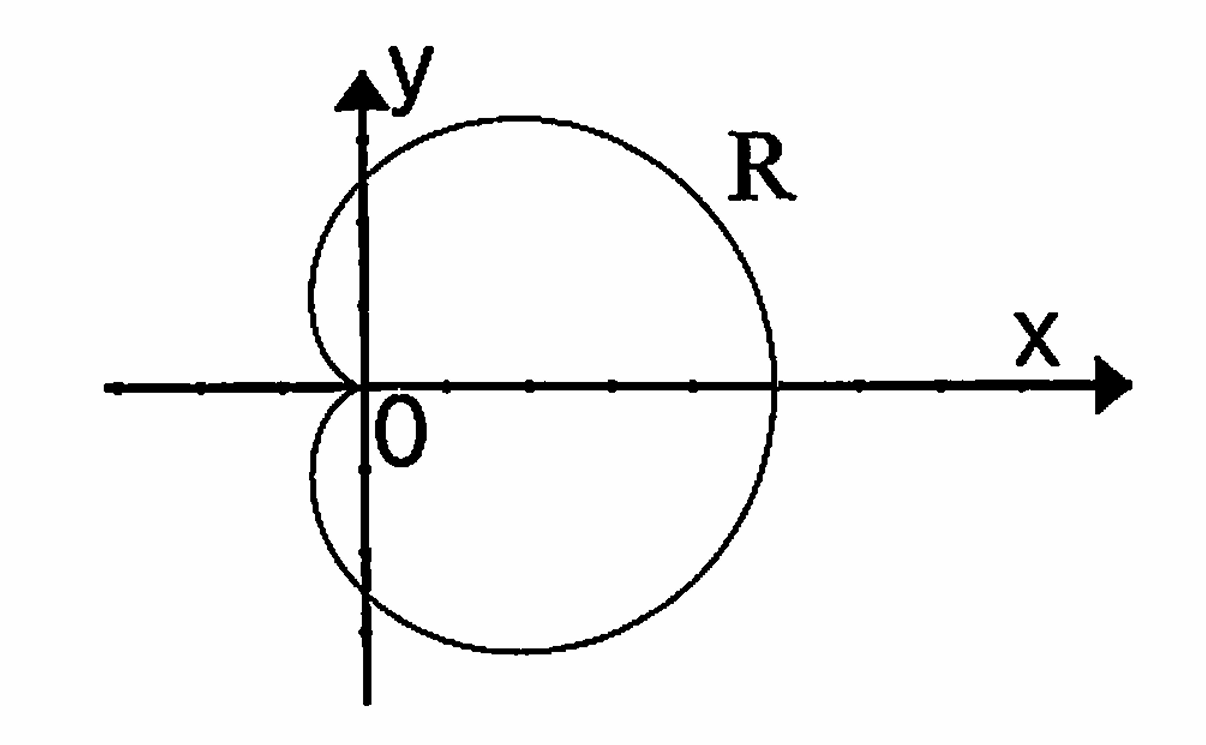
\includegraphics[width=.35\linewidth]{./src/fig/Basic/B_2019_autumn_2-4.png}
  \end{figure}
}
\begin{ans*}
  ${}$
  与えられた積分は$xyz$空間で$R$上で$z=0$と$z=y$で囲まれた部分の積分を表す。

  ここで、$x = k\in\bbR$での切断面について
  $z=y$は原点$(x,y,z)=(k,0,0)$で対称であるので求める積分は
  \begin{gather}
    I = \iint_{R}y\,dxdy = 0
  \end{gather}
\end{ans*}
\begin{other*}
  あるいは極座標変換によって
  \begin{align}
    I
    &= \iint_{R}y\,dxdy \\
    &= \int_{0}^{2\pi}\int_{0}^{2a(1-\cos\grt)}\bigl(r^2 \sin\grt\bigr)drd\grt \\
    &= \int_{0}^{2\pi}d\grt \left[\frac{1}{3}r^3 \sin\grt\right]_{0}^{2a(1+\cos\grt)} \\
    &= \frac{4a^2}{3}\int_{0}^{2\pi} \sin\grt(1+\cos\grt)^2\,d\grt \\
    &= 0
  \end{align}
\end{other*}

\subsection{線形代数}
\prob{
  ベクトル
  \begin{gather}
    \bv_{1} = \Bmat{1 \\ 1 \\ 1},\,\bv_{2} = \Bmat{1 \\ 2 \\ -1}
  \end{gather}
  が与えられるとき、以下の問いに答えよ。
  \begin{enumerate}[label=(\arabic*)]
    \item ベクトル
    \begin{gather}
      \bu = \Bmat{3 \\ 4 \\ 1}
    \end{gather}
    が$\bv_{1}$と$\bv_{2}$の線形結合で表されることを示せ。
    \item ベクトル
    \begin{gather}
      \bw = \Bmat{1 \\ 0 \\ 0}
    \end{gather}
    が$\bv_{1}$と$\bv_{2}$の線形結合で表されないことを示せ。
  \end{enumerate}
}
\begin{ans*}
  ${}$
  \begin{enumerate}[label=(\arabic*)]
    \item
    \begin{gather}
      \bu = 2\bv_{1} + \bv_{2}
    \end{gather}
    と表せる。
    \item $\bw$が$\bv_{1}$と$\bv_{2}$の線形結合で表されないので、
    ベクトルの組$\bv_{1},\,\bv_{2},\,\bw$が一次独立である、すなわち
    このベクトルを並べた行列$\bP := [\bv_{1},\,\bv_{2},\,\bw]$
    の階数について$\rank\bP=3$となることを示す。
    $\bP$について次の行基本変形
    \begin{align}
      \bP
      &\lra \bmat{
        1 & 1 & 1 \\
        1 & 2 & 0 \\
        1 & -1 & 0
      } \\
      &\lra \bmat{
        1 & 1 & 1 \\
        0 & 1 & -1 \\
        0 & -2 & -1
      } \\
      &\lra \bmat{
        1 & 1 & 1 \\
        0 & 1 & -1 \\
        0 & 0 & 1
      } \\
      &\lra \bmat{
        1 & 0 & 0 \\
        0 & 1 & 0 \\
        0 & 0 & 1
      }
    \end{align}
    より、$\rank\bP = 3$であり、
    たしかに$\bw$は$\bv_{1}$と$\bv_{2}$の線形結合で表されない。
  \end{enumerate}
\end{ans*}

ここで、ベクトルの組$\bv_{1},\,\bv_{2},\,\bw$が一次独立であることと、
$\bP := [\bv_{1},\,\bv_{2},\,\bw]$
の階数について$\rank\bP=3$となることが同値であることを示しておきます。

\begin{proof}
  行列$\bP$を、\dm{\bP\colon \bbR^3\lra\bbR^3\colon \bx\lra\bP\bx}という線形写像とすると、
  \begin{align}
    &\text{ベクトルの組}\bv_{1},\,\bv_{2},\,\bw \text{が一次独立である} \notag \\
    &\eqa \text{「}\bv_1x_1 + \bv_2x_2 + \bw x_3 = \bP\bx = \bzv \eqa \bx = \bzv\text{」} \\
    &\eqa \Ker\bP = \Dset{\bx\in\bbR^3\relmiddle \bP\bx = \bzv} = \{\bzv\} \\
    &\eqa \dim\Ker\bP = 0 \\
    &\eqa \rank\bP = n = 3\quad\text{($\because$ 次元定理)}
  \end{align}
  より、行列$\bP$の列ベクトルが一次独立であることと$\rank\bP = n$であることは同値である。
\end{proof}


\prob{
  行列
  \begin{gather}
    \bA = \bmat{
      -1 & 2 & 2 \\
      2 & -1 & 2 \\
      2 & 2 & -1
    }
  \end{gather}
  について、以下の問いに答えよ。
  \begin{enumerate}[label=(\arabic*)]
    \item 固有値と、それぞれの重複度を求めよ。
    \item 各固有値に対応する固有ベクトルを求めよ。
    \item $\bA$が対角化できることを示せ。
    \item 固有空間の次元を答えよ。
  \end{enumerate}
}

\begin{ans*}
  ${}$
  \begin{enumerate}[label=(\arabic*)]
    \item 固有方程式$\det(\bA - \grl\bE) = 0$より
    \begin{gather}
      (-1-\grl)(-1-\grl)(-1-\grl) + 8 + 8 - 3\tm(-1-\grl)\tm 4 = -(\grl + 3)^2(\grl - 3) = 0 \\
      \grl = 3, \, -3
    \end{gather}
    また、$\grl = 3$の重複度は1、$\grl = -3$の重複度は2である。
    \item
    \begin{enumerate}[label=(\roman*)]
      \item $\grl = 3$のとき固有ベクトル$\bu=\{x,\, y,\, z\}^{\top}$は
      \begin{gather}
        \bmat{
          -4 & 2 & 2 \\
          2 & -4 & 2 \\
          2 & 2 & -4
        }\bu = \bzv \\
        \begin{dcases*}
          -4x +  2y + 2z = 0 \\
          2x -4y + 2z = 0 \\
          2x + 2y -4z = 0
        \end{dcases*} \\
        \bu = t\Bmat{
          1 \\ 1 \\ 1
        }\quad(t\in\bbR\backslash\{0\})
      \end{gather}
      よって、このときの正規化された固有ベクトル$\bu_{1}$は
      \begin{gather}
        \bu_{1} = \frac{1}{\sqrt{3}}\Bmat{
          1 \\ 1 \\ 1
        }
      \end{gather}
      \item $\grl = -3$のとき固有ベクトル$\bu = \{x,\,y,\,z\}^{\top}$は
      \begin{gather}
        \bmat{
          2 & 2 & 2 \\
          2 & 2 & 2 \\
          2 & 2 & 2 \\
        }\bu = \bzv \\
        2x + 2y + 2z = 0 \\
        \bu = s \Bmat{
          -1 \\ 1 \\ 0
        } + t\Bmat{
          -1 \\ 0 \\ 1
        }\quad (s,t\in\bbR \land (s,t)\neq(0,0))
      \end{gather}
      よって、正規化された固有ベクトルとしては$s=0$と$t=0$を考えれば
      一次独立である2つがとれて、それを正規化したものを$\bu_{2},\,\bu_{3}$と表すと
      \begin{gather}
        \bu_{2} = \frac{1}{\sqrt{2}}\Bmat{
          -1 \\ 1 \\ 0
        },\quad
        \bu_{3} = \frac{1}{\sqrt{2}}\Bmat{
          -1 \\ 0 \\ 1
        }
      \end{gather}
    \end{enumerate}
    \item $\bA\in\bbR^{3\tm3}$で、固有ベクトルは3つあるので対角化可能である。\\
    実際、行列$\bP :=[\sqrt{3}\bu_{1},\,\sqrt{2}\bu_{2},\,\sqrt{2}\bu_{3}]$について
    \begin{align}
      [\bP|\bE]
      &= \left[\begin{array}{ccc|ccc}
        1 & -1 & -1 & 1 & 0 & 0 \\
        1 & 1 & 0 & 0 & 1 & 0 \\
        1 & 0 & 1 & 0 & 0 & 1 \\
      \end{array}\right] \\
      &\lra \left[\begin{array}{ccc|ccc}
        1 & -1 & -1 & 1 & 0 & 0 \\
        0 & 2 & 1 & -1 & 1 & 0 \\
        0 & 1 & 2 & -1 & 0 & 1 \\
      \end{array}\right] \\
      &\lra \left[\begin{array}{ccc|ccc}
        1 & -1 & -1 & 1 & 0 & 0 \\
        0 & 1 & 1/2 & -1/2 & 1/2 & 0 \\
        0 & 0 & 3/2 & -1/2 & -1/2 & 1 \\
      \end{array}\right] \\
      &\lra \left[\begin{array}{ccc|ccc}
        1 & -1 & -1 & 1 & 0 & 0 \\
        0 & 1 & 1/2 & -1/2 & 1/2 & 0 \\
        0 & 0 & 1 & -1/3 & -1/3 & 2/3 \\
      \end{array}\right] \\
      &\lra \left[\begin{array}{ccc|ccc}
        1 & -1 & -1 & 1 & 0 & 0 \\
        0 & 1 & 0 & -1/3 & 2/3 & -1/3 \\
        0 & 0 & 1 & -1/3 & -1/3 & 2/3 \\
      \end{array}\right] \\
      &\lra \left[\begin{array}{ccc|ccc}
        1 & 0 & 0 & 1/3 & 1/3 & 1/3 \\
        0 & 1 & 0 & -1/3 & 2/3 & -1/3 \\
        0 & 0 & 1 & -1/3 & -1/3 & 2/3 \\
      \end{array}\right] \\
      &=[\bE|\bP^{-1}]
    \end{align}
    より$\bP^{-1}\bA\bP$は
    \begin{align}
      \bP^{-1}\bA\bP
      &= \bmat{
        1 & 1 & 1 \\
        1 & -2 & 1 \\
        1 & 1 & -2
      }\bP \\
      &= \bmat{
        3 & 0 & 0 \\
        0 & -3 & 0 \\
        0 & 0 & -3
      }
    \end{align}
    であるので、たしかに対角化できる。
  \end{enumerate}

  あるいは正規化されたままのベクトルを並べた行列$\bQ:=[\bu_{1},\,\bu_{2},\,\bu_{3}]$について
  \begin{align}
    [\bQ|\bE]
    &= \left[\begin{array}{ccc|ccc}
      1/\sqrt{3} & -1/\sqrt{2} & -1/\sqrt{2} & 1 & 0 & 0\\
      1/\sqrt{3} & 1/\sqrt{2} & 0 & 0 & 1 & 0\\
      1/\sqrt{3} & 0 & 1/\sqrt{2} & 0 & 0 & 1
    \end{array}\right] \\
    &\lra \left[\begin{array}{ccc|ccc}
      1 & -\sqrt{3}/\sqrt{2} & -\sqrt{3}/\sqrt{2} & \sqrt{3} & 0 & 0 \\
      0 & 2/\sqrt{2} & 1/\sqrt{2} & -1 & 1 & 0\\
      0 & 1/\sqrt{2} & 2/\sqrt{2} & -1 & 0 & 1
    \end{array}\right] \\
    &\lra \left[\begin{array}{ccc|ccc}
      1 & -\sqrt{3}/\sqrt{2} & -\sqrt{3}/\sqrt{2} & \sqrt{3} & 0 & 0 \\
      0 & 1 & 1/2 & -1/\sqrt{2} & 1/\sqrt{2} & 0\\
      0 & 0 & 3/2\sqrt{2} & -1/2 & -1/2 & 1
    \end{array}\right] \\
    &\lra \left[\begin{array}{ccc|ccc}
      1 & -\sqrt{3}/\sqrt{2} & -\sqrt{3}/\sqrt{2} & \sqrt{3} & 0 & 0 \\
      0 & 1 & 1/2 & -1/\sqrt{2} & 1/\sqrt{2} & 0\\
      0 & 0 & 1 & -\sqrt{2}/3 & -\sqrt{2}/3 & 2\sqrt{2}/3
    \end{array}\right] \\
    &\lra \left[\begin{array}{ccc|ccc}
      1 & -\sqrt{3}/\sqrt{2} & 0 & 2\sqrt{3}/3 & -\sqrt{3}/3 & 2\sqrt{3}/3 \\
      0 & 1 & 0 & -\sqrt{2}/3 & 2\sqrt{2}/3 & -\sqrt{2}/3 \\
      0 & 0 & 1 & -\sqrt{2}/3 & -\sqrt{2}/3 & 2\sqrt{2}/3
    \end{array}\right] \\
    &\lra \left[\begin{array}{ccc|ccc}
      1 & 1 & 0 & \sqrt{3}/3 & \sqrt{3}/3 & \sqrt{3}/3 \\
      0 & 1 & 0 & -\sqrt{2}/3 & 2\sqrt{2}/3 & -\sqrt{2}/3 \\
      0 & 0 & 1 & -\sqrt{2}/3 & -\sqrt{2}/3 & 2\sqrt{2}/3
    \end{array}\right]
  \end{align}
  より$\bQ^{-1}\bA\bQ$は
  \begin{align}
    \bQ^{-1}\bA\bQ
    &= \bmat{
      \sqrt{3} & \sqrt{3} & \sqrt{3} \\
      \sqrt{2} & -2\sqrt{2} & \sqrt{2} \\
      \sqrt{2} & \sqrt{2} & -2\sqrt{2}
    }\bQ \\
    &= \bmat{
      3 & 0 & 0 \\
      0 & -3 & 0 \\
      0 & 0 & -3
    }
  \end{align}
  であるので、たしかに対角化できる。
  \item 行列$\bA$の固有値$\grl$に対する固有空間$W_{\grl}$とは固有ベクトル$\bu$を用いて
  \begin{gather}
    W_{\grl} = \Dset{t\bu\relmiddle t\in\bbR\backslash \{0\} } \cup\{\bm{0}\} = \Dset{\bx\in\bbR^{3}\relmiddle \bA\bx = \grl\bx}
  \end{gather}
  を満たす$\bbR^3$の部分空間である。
  すなわち、$\bA - \grl\bE$を線形写像$\bP$としたとき、固有空間は
  \begin{align}
    W_{\grl}
    &= \Dset{\bx\in\bbR^{3}\relmiddle (\bA - \grl\bE)\bx = \bzv} \\
    &= \Dset{\bx\in\bbR^{3}\relmiddle \bP\bx = \bzv} \\
    &= \Ker\bP
  \end{align}
  であるので$\bP$の核である。
  \begin{enumerate}[label=(\roman*)]
    \item $\grl = 3$のとき、
    \begin{gather}
      W_{3} = \Ker\bmat{
        -4 & 2 & 2 \\
        2 & -4 & 2 \\
        2 & 2 & -4
      } = \Dset{
        t\{1, 1, 1\}^{\top} \relmiddle t\in\bbR
      }
    \end{gather}
    よって、$\grl=3$の固有空間$W_{3}$の次元は$1$。
    \item $\grl = 3$のとき、
    \begin{gather}
      W_{-3} = \Ker\bmat{
        2 & 2 & 2 \\
        2 & 2 & 2 \\
        2 & 2 & 2 \\
      } = \Dset{
        s\{-1, 1, 0\}^{\top} + t\{-1, 0, 1\}^{\top} \relmiddle s, t\in\bbR
      }
    \end{gather}
    ここで、$\{-1, 1, 0\}^{\top},\,\{-1, 0, 1\}^{\top}$は一次独立だから、
    $\grl=3$の固有空間$W_{-3}$の次元は$2$。
  \end{enumerate}
\end{ans*}



\prob{
  3次の正方行列$\bA,\,\bB$の行列式が、それぞれ$\det\bA = 3,\,\det\bB = -2$のとき、
  (a)\,$\det(\bA\bB)$、(b)\,$\det(\bA^{-1}\bB)$、(c)\,$\det(2\bA)$を求めよ。
}
\begin{ans*}
  ${}$
  \begin{enumerate}[label=(\alph*)]
    \item \dm{\det(\bA\bB) = \det\bA\det\bB = -6}
    \item \dm{\det(\bA^{-1}\bB) = \frac{\det\bB}{\det\bA} = -\frac{2}{3}}
    \item \dm{\det(2\bA) = 2^3 \cdot 3 = 24}
  \end{enumerate}
\end{ans*}
